\documentclass[a4paper]{article}

%% Language and font encodings
\usepackage{polski}
\usepackage[utf8]{inputenc}
\usepackage[T1]{fontenc}
\usepackage{pdfpages}
\usepackage{indentfirst}

% Adjust penalties
\brokenpenalty=1000
\clubpenalty=1000
\widowpenalty=1000

%% Sets page size and margins
\usepackage[a4paper]{geometry}

%% Useful packages
\usepackage{amsmath}
\usepackage{graphicx}
\usepackage[colorlinks=true, allcolors=blue]{hyperref}
\usepackage{booktabs}
\usepackage{cancel}
\usepackage{tikz}

\usepackage{float}

\renewcommand\thesection{\arabic{section}.}
\renewcommand\thesubsection{\arabic{section}.\arabic{subsection}.}
\renewcommand\thesubsubsection{\arabic{section}.\arabic{subsection}. \arabic{subsubsection}.}

% The following commands are not supported in PSTricks at present
% We define them conditionally, so when they are implemented,
% this pgf file will use them.
\ifx\du\undefined
  \newlength{\du}
\fi
\setlength{\du}{15\unitlength}

\newcommand{\Vsp}[1]{\vtop to #1 {}}
\newcommand{\Hsp}[1]{\hbox to #1 {}}
\newcommand{\Small}{\scriptsize}

\title{Sprawozdanie nr 2}
\date{}


\begin{document}

\begin{center}
\begin{tabular}{|p{5.5cm}|l|l|c|}
    \hline
	% Row 1.1  
	    Wydział \Vsp{4mm} &
	    \multicolumn{1}{|l}{Dzień} &
	    poniedziałek $17^{15} - 19^{30}$ &
	    Nr zespołu \\
	% Row 1.2
	    \mbox{\small{Matematyki i Nauk Informatycznych}} &
	    \multicolumn{1}{|l}{Data}  &
	    &
	    \multicolumn{1}{c|}{\Large{18}} \\
    
    \hline
	% Row 2.1 
	    Nazwisko i Imię: &
	    \Small Ocena z przygotowania &
	    \Small Ocena ze sprawozdania &
	    \Small Ocena Końcowa \\
	% Rows 2.2-2.4
	    1. Jasiński Bartosz & & &\\
	    2. Sadłocha Adrian & & & \\
	    3. Wódkiewicz Andrzej & & & \\

    \hline
    % Row 3.1
	    \multicolumn{2}{|l|}{Prowadzący \Vsp{4mm}} &
	    \multicolumn{2}{|l|}{Podpis prowadzącego} \\  
    % Row 3.2
    	\multicolumn{2}{|l|}{dr inż. Jarosław Judyk} &
    	\multicolumn{2}{|l|}{} \\    	
    \hline
\end{tabular}
\label{pieczatka}
\end{center}

{\let\newpage\relax\maketitle}  % stolen from: https://tex.stackexchange.com/questions/86249/maketitle-text-before-title
\setcounter{secnumdepth}{2}


\section{Opis ćwiczenia}
Ćwiczenie złożone było z dwóch części:
\begin{enumerate}
	\item{Badanie anharmoniczności drgań wahadła matematycznego}
	\item{Wyznaczanie przyspieszenia ziemskiego za pomocą wahadła różnicowego}
\end{enumerate}


\subsection{Wstęp teoretyczny}

\textbf{Wahadłem matematycznym płaskim} nazywamy punkt materialny, poruszający się
ruchem okrężnym w jednorodnym polu grawitacyjnym. Praktyczną realizacją tego pojęcia
jest obciążnik (najczęściej kulka) o małych rozmiarach, zamocowany do nierozciągliwej
nici o bardzo małej, pomijalnej masie (Rysunek \ref{wahadlo_matematyczne}). 

\begin{figure}[h]
\caption{Wahadło matematyczne}
%TODO Insert graphic here
\label{wahadlo_matematyczne}
\end{figure}

Siłę ciężkości $\vec{F}_g = m\vec{g}$ działającą na ciężarek możemy rozłożyć na
składową radialną $F_g \cos \theta$ oraz styczną do toru ruchu wahadła $F_g \sin \theta$.
Składowa styczna wpływa na powrót ciężarka do położenia równowagi, gdyż działa ona
zawsze przeciwnie do jego wychylenia. Z drugiej zasady dynamiki Newtona mamy więc:

\begin{align*}
 ma &= -mg\sin\theta \\
 \frac{d^2S}{dt^2} &= -g\sin\theta
\end{align*}

Ponieważ $S = l \cdot \theta$:

\[ \frac{d^2\theta}{dt^2} = -\frac{g}{l}\sin\theta \]

Nie istnieje analityczne rozwiązanie tego równania różniczkowego. Dla małych kątów
można uprościć powyższy wzór, zakładając, że \, $\sin\theta \approx \theta$ \,
-- wtedy równanie różniczkowe daje się rozwiązać analitycznie. W rezultacie otrzymujemy,
że \textbf{dla wahadła matematycznego poruszającego się w zakresie małych kątów}
(przy założeniu $\theta(0) = \theta_{max}$):

\[ \theta(t) = \theta_{max}\cos\left(\sqrt{\frac{g}{l}}\right), \] 

czyli ruch \textbf{jest harmoniczny}, a okres tego ruchu wynosi

\[ T = 2\pi~\sqrt{\frac{l}{g}} \]


W ogólności (bez założenia małych wychyleń), korzystając z rozwinięcia funkcji $sin$
w szereg, możemy finalnie otrzymać zależność okresu drgań wahadła $T$ od kąta
maksymalnego wychylenia $\theta_{max}$:

\[ 
	T = 2\pi ~ \sqrt[]{\frac{l}{g}}~f(\theta_{max}) 
, \enskip \text{gdzie} \enskip \enskip 
f(\theta_{max}) = 
	\sum\limits_{i=0}^{\infty} 
		\left[ \frac{(2n)!}{(2^nn!)^2} \right]^2 
			\sin^{2n}\left(\frac{\theta_{max}}{2} \right) \]

Ruch wahadła matematycznego jest więc w ogólności \textbf{anharmoniczny} -- okres
jest zależny od amplitudy.



\subsection{Układ pomiarowy}
Do przeprowadzenia obu części ćwiczenia posłużono się układem pomiarowym,
przedstawionym na rysunku \ref{uklad_pomiarowy}. Do ruchomego elementu 
połączonego z nieruchomym statywem przymocowana była długa, nierozciągliwa nitka, 
o znikomo małej masie, z zamocowanym na jej końcu metalowym obciążnikiem. 
Ruch elementu w pionie pozwalał modyfikować długość wahadła. Do statywu 
przytwierdzony był również kątomierz oraz linijka, służące do pomiaru kolejno:
kąta maksymalnego wychylenia wahadła oraz zmiany długości wahadła różnicowego.
Pod statywem znajdował się elektroniczny układ pomiarowy, złożony z fotokomórki
oraz modułu sterowania, za pomocą którego mierzony był okres wahadła.


\begin{figure}[h]
\caption{Schemat układu pomiarowego}
%TODO Insert graphic here
\label{uklad_pomiarowy}
\end{figure}


\section{Pomiary i obliczenia}
\subsection{Badanie zależności okresu drgań wahadła od kąta wychylenia}


\begin{table}[h]
\centering
	\begin{tabular}{rrrrrrr}
	\toprule
	{} &$2T(\alpha=5^\circ)$ &$2T(10^\circ)$ &$2T(15^\circ)$ &$2T(20^\circ)$ &$2T(25^\circ)$ &$2T(30^\circ)$ \\
	\midrule
	1 &  2.6285 &  2.6343 &  2.6368 &  2.6454 &  2.6585 &  2.6701 \\
	2 &  2.6295 &  2.6346 &  2.6359 &  2.6463 &  2.6589 &  2.6711 \\
	3 &  2.6295 &  2.6344 &  2.6402 &  2.6467 &  2.6582 &  2.6714 \\
	4 &  2.6307 &  2.6366 &  2.6394 &  2.6470 &  2.6590 &  2.6709 \\
	5 &  2.6296 &  2.6358 &  2.6408 &  2.6467 &  2.6578 &  2.6701 \\
	6 &  2.6286 &  2.6350 &  2.6404 &  2.6463 &  2.6593 &  2.6685 \\
	7 &  2.6285 &  2.6342 &  2.6396 &  2.6463 &  2.6574 &  2.6698 \\
	8 &  2.6303 &  2.6350 &  2.6401 &  2.6477 &  2.6588 &  2.6696 \\
	9 &  2.6287 &  2.6352 &  2.6395 &  2.6476 &  2.6583 &  2.6694 \\
	10 &  2.6298 &  2.6350 &  2.6396 &  2.6485 &  2.6584 &  2.6708 \\
	\midrule
	$2\overline{T}$& 2.62937 & 2.63501 & 2.63923 & 2.64685 & 2.64685 & 2.67017 \\ 
	$s(2T)$ & 0.00078 & 0.00074 & 0.00160 & 0.00089 & 0.00057 & 0.00089 \\
	\bottomrule
\end{tabular}
\caption{Seria pomiarów czasu trwania 2 okresów wahadła w zależności od kąta wychylenia}
\label{pomiary_1}
\end{table}


\begin{figure}[h!]
\centering
	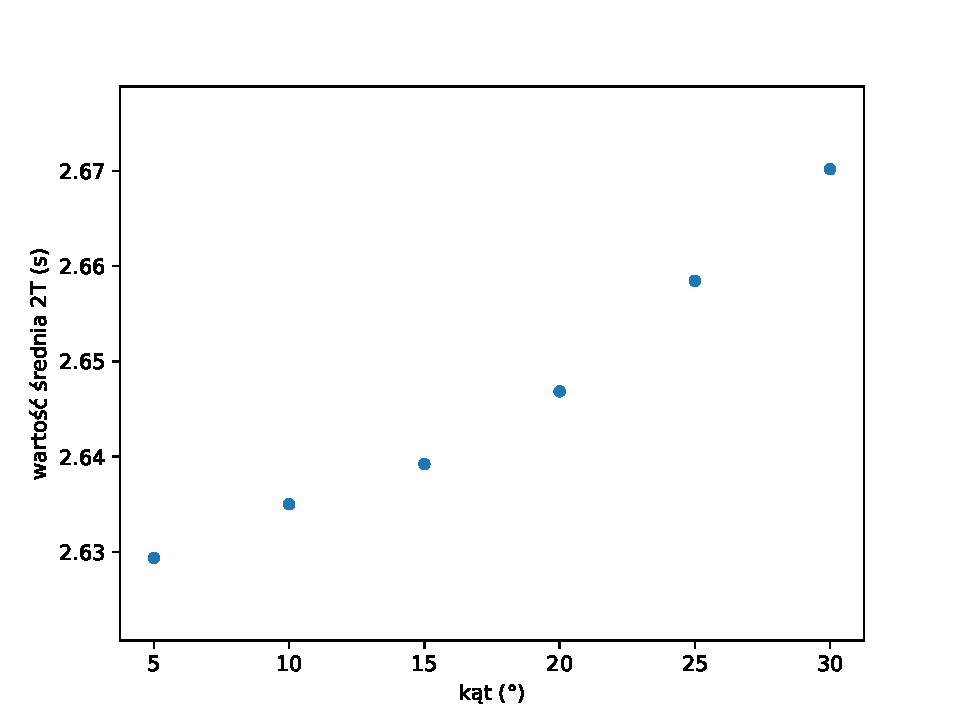
\includegraphics[scale=0.8]{wykres-1_0.pdf}
\caption{Wartość średnia 2 okresów wahadła w zależności od maksymalnego kąta wychylenia}
\label{wykres_1}
\end{figure}


\begin{figure}[h!]
\centering
	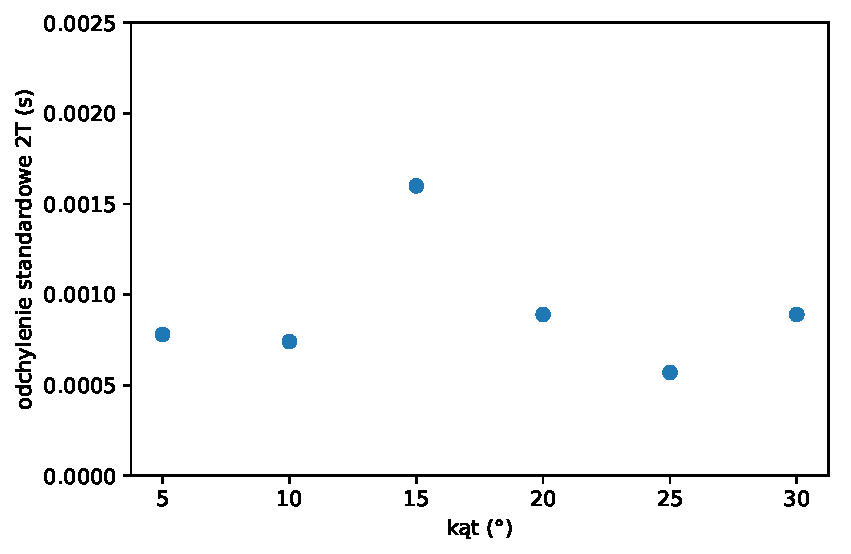
\includegraphics[scale=0.85]{wykres-2_1.pdf}
\caption{Odchylenie standardowe 2 okresów wahadła w zależności od maksymalnego kąta wychylenia}
\end{figure}

\subsection{Badanie zależności okresu drgań wahadła od zmian długości}
\subsubsection{Pomiary okresu dla wahadła różnicowego i małego kąta}



\begin{table}[h!]
\centering
	\begin{tabular}{lrrrrrr}
	\toprule
	{} & $l$ (mm) $=Y$ &  $2T$ (s) & \small$1000T^2/4\pi^2$\normalsize$=X$ & $X^2$ & $Y^2$ & $XY$ \\
	\midrule
	1 &     480 &  2.6325 &  43.885094 &  1925.9015 &  230400 &  21064.845 \\
	2 &     460 &  2.6918 &  45.884484 &  2105.3859 &  211600 &  21106.863 \\
	3 &     440 &  2.7515 &  47.942349 &  2298.4688 &  193600 &  21094.634 \\
	4 &     420 &  2.8101 &  50.006196 &  2500.6196 &  176400 &  21002.602 \\
	5 &     400 &  2.8676 &  52.073578 &  2711.6575 &  160000 &  20829.431 \\
	6 &     380 &  2.9218 &  54.060647 &  2922.5536 &  144400 &  20543.046 \\
	\midrule
	$\Sigma$ & 2580 & 16.6753 & 293.852348 & 14464.5869 & 1116400 & 125641.421 \\
	\end{tabular}
\caption{Pomiary 2 okresów wahadła dla maksymalnego kąta wychylenia $\theta_{max} = 10^\circ$ w  zależności od $l$ wraz z obliczeniami do wyznaczenia regresji liniowej}
\label{pomiary_2}
\end{table}



\begin{figure}[h!]
\centering
	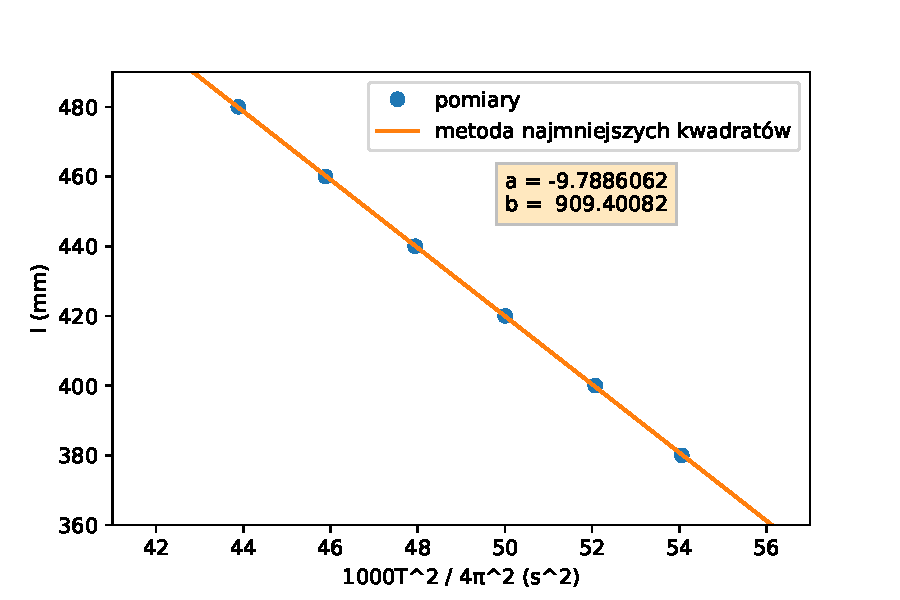
\includegraphics[scale=0.85]{wykres-3_0.pdf}
\caption{Regresja liniowa metodą najmniejszych kwadratów dla $\theta_{max} = 10^\circ$}
\label{regresja_10}
\end{figure}


\subsubsection{Pomiary okresu dla wahadła różnicowego i dużego kąta}



\begin{table}[h]
\centering

	\begin{tabular}{lrrrrrr}
	\toprule
		{} & $l$ (mm) $=Y$ &  $2T$ (s) & \small$1000T^2/4\pi^2$\normalsize$=X$ & $X^2$ & $Y^2$ & $XY$ \\
	\midrule
	1 &     480 &  2.6582 &  44.74614 &  2002.2170 &  230400 &  21478.147 \\
	2 &     460 &  2.7160 &  46.71322 &  2182.1249 &  211600 &  21488.081 \\
	3 &     440 &  2.7764 &  48.81399 &  2382.8056 &  193600 &  21478.136 \\
	4 &     420 &  2.8339 &  50.85683 &  2586.4132 &  176400 &  21359.869 \\
	5 &     400 &  2.8918 &  52.95620 &  2804.3591 &  160000 &  21182.480 \\
	6 &     380 &  2.9494 &  55.08681 &  3034.5566 &  144400 &  20932.988 \\
	\midrule
	$\Sigma$ & 2580 & 16.8257 & 299.17319& 14992.4764 & 1116400 & 127919.701 \\
	\bottomrule
	\end{tabular}
	
\caption{Pomiary 2 okresów wahadła dla maksymalnego kąta wychylenia $\theta_{max} = 25^\circ$ w  zależności od $l$ wraz z obliczeniami do wyznaczenia regresji liniowej}
\end{table}

\begin{figure}[h!]
\centering
	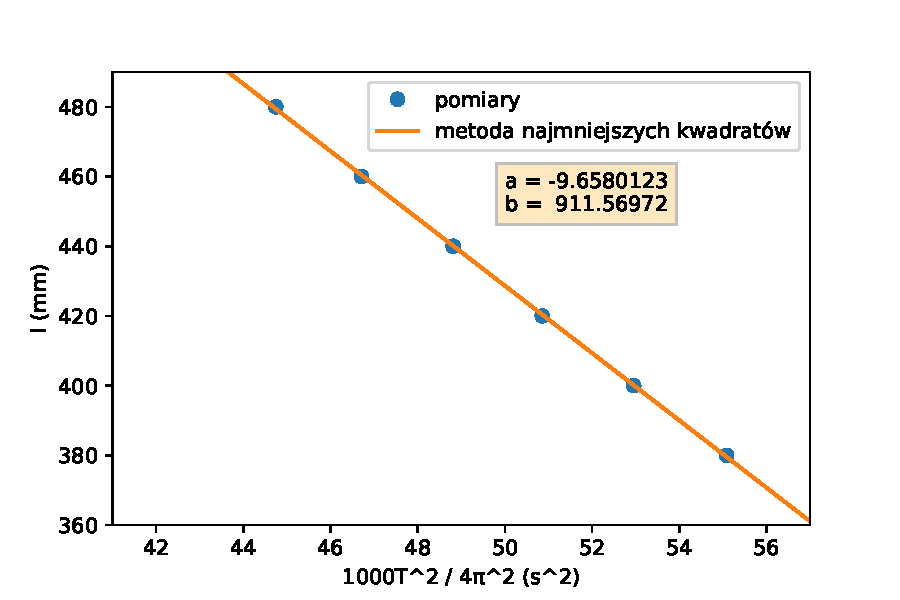
\includegraphics[scale=0.85]{wykres-4_0.pdf}
\caption{Regresja liniowa metodą najmniejszych kwadratów dla $\theta_{max} = 25^\circ$}
\label{regresja_25}
\end{figure}



\end{document}